\section{Coatings}
\label{sec:coatingsintro}
Optical Interference Coatings (OIC) are used in all optics of an interferometer but those deposited on the mirrors of the Fabry-Perot cavities are need to have the highest optical and mechanical performance. OIC are used to produce High Reflecting (HR) or Anti Reflecting (AR) surfaces. The transmission have to be specified over multiple wavelengths depending on the control scheme adopted by the detector. \\

The optical properties of the OIC that are relevant for a GW detectors are: Transmission $T(\lambda)$; absorption $\alpha(\lambda)$; Total Integrated Scatter (TIS); Bidirectional Reflectance Distribution Function (BRDF); wave form distortion; density of point defects. All these parameters need to have a specific uniformity over the optics surface. \\
The mechanical properties relevant for a GW detector are: mechanical loss angle $\phi$ for each elastic constant; the elastic constants; the internal stress $\sigma$; the adhesion to the substrate; thermal expansion coefficients; thermo elastic coefficients. Mechanical properties uniformity follow that of the optical properties.\\ 

Three main technologies are possible:\\
a) amorphous materials; \\
b) crystalline materials; \\
c) nano structured surfaces (coating-free optics). \\

New type of coatings are required for 3 potential wavelengths (1064 nm, 1550 nm and 2 $\mu$m), for 3 temperature ranges (room temperature, 120 K and below 20 K), for 3 different substrates (silica, sapphire and silicon) and for diameters ranging between 35 cm and 60 cm. \\

R\&D activities on materials, that are concentrated mostly on mechanical losses and absorption, have to go in parallel with the development of the deposition technology that should take care of all the other optical and mechanical parameters and that guaranties the uniformity of optical performance on large diameters.

There are 4 large areas of development in the coating research: Metrology, Materials, Deposition Technology and Fundamental Processes. In the following table a summary of the various research lines is provided:
%
\begin{longtable}{|p{0.25\textwidth}|p{0.3\textwidth}|p{0.45\textwidth}|}
\caption{Bla bla\label{tab:characterization}} \\
\hline\hline
\endfirsthead
\caption[]{(continued)}\\
\hline\hline
\endhead
{\sc Metrology} & Thermomechanical & Elastic Constants \\\cline{3-3}
 & & Internal stress \\\cline{3-3}
 & & Thermal coefficients \\\cline{2-3}
 & Mechanical Loss & Clamped systems \\\cline{3-3}
 & & Nodal systems \\\cline{3-3}
 & & Suspended systems \\\cline{2-3}
 & TN measurements & AF cantilevers \\\cline{3-3}
 & & Doubble paddle \\\cline{3-3}
 & & On mirrors \\\cline{2-3}
 & Optical characterization & Complex indeces \\\cline{3-3}
 & & Thermal coefficients \\\cline{3-3}
 & & Scattering \\\cline{3-3}
 & & Point defects statistics\\\hline\hline 
{\sc Materials} & Amorphous & Oxides \\\cline{3-3}
 & & Nitrides \\\cline{3-3}
 & & Fluorides \\\cline{3-3}
 & & Silicon \\\cline{3-3}
 & & Co-sputtered alloys \\\cline{3-3}
 & & Nano layered alloys \\\cline{2-3}
 & Crystallines & AlGaAs \\\cline{3-3}
 & & AlGaP \\\cline{3-3}
 & & AlGaN \\\cline{2-3}
 & Nano structured & On silicon \\\hline\hline
{\sc Deposition} & Amorphous & Uniformity \\\cline{3-3}
{\sc Technology} & & Parameters optimization \\\cline{3-3}
 & & Poit defect/scatterer reduction \\\cline{3-3}
 & & Post-deposition corrective coatings \\\cline{3-3}
 & & Elevated temperature deposition \\\cline{3-3}
 & & Annealing \\\cline{3-3}
 & & Nano layered structures \\\cline{2-3}
 & Crystallines & Uniformity \\\cline{3-3}
 & & Parameters optimization \\\cline{3-3}
 & & Point defect reduction \\\cline{3-3}
 & & Coatings transfert \\\cline{3-3}
 & & Adhesion \\\hline\hline
{\sc Fundamental} & Amorphous & Ultrastable glasses \\\cline{3-3}
{\sc Processes} & & Deposition processes \\\cline{3-3}
 & & Correlation loss-structure \\\cline{3-3}
 & & Correlation absorption-structure \\\cline{3-3}
 & & Role of contaminants \\\cline{2-3}
 & Crystallines & Dislocations \\\cline{3-3}
 & & Role of contaminants \\\cline{3-3}
 & & Effect of stress \\\cline{3-3}
 & & Mechanical losses from bonding \\\hline\hline
\end{longtable}
%
\subsection{Current State of the Art}
The materials used in the Advanced detectors have the following reference values for losses~\cite{Granata_2016} $\phi$ and extintion coefficient~\cite{Pinard_2017} $\kappa$ (it is linked to the attenuation through the relation $\alpha = 4\pi\,\kappa\,d/\lambda$ where $d$ is the thickness): \\
%
\begin{center}
\begin{tabular}{l|c|c|c}
            & $\phi$ & $\kappa$ & n \\ \hline
 SiO$_2$                 & $4.5\times 10^{-5}$ & $10^{-8}$        & 1.442  \\ \hline
 TiO$_2\,$Ta$_2$O$_5$    & $2.4\times 10^{-4}$ & $2\times 10^{-8}$ & 2.07  \\ \hline
\end{tabular}
\end{center}
%

%
\begin{minipage}{0.35\textwidth}
\end{minipage}\hfill
\begin{minipage}{0.6\textwidth}
\vspace{-0.cm}
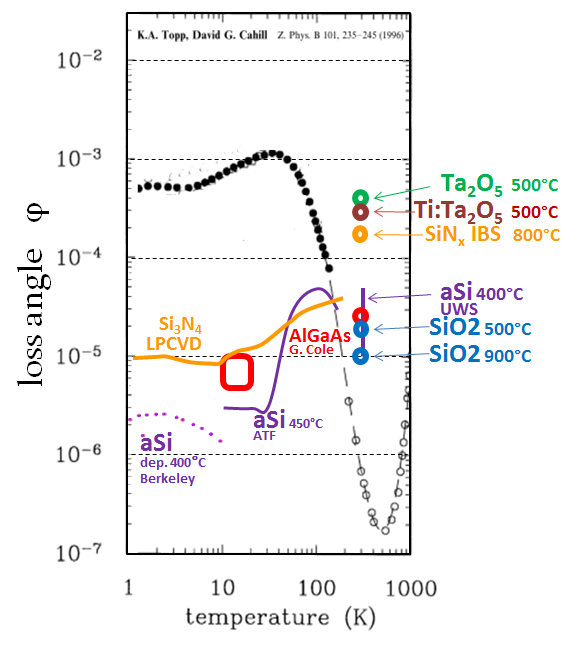
\includegraphics[width=\textwidth]{Figures/Status_coatings.png} \label{fig:coatinglosstatus}
\vspace{-0.5cm}
\captionof{figure}{Mechanical losses of the materials used in the Advanced detector and of some of the most promising materials. The measurements were done in the acoustic band.} \vspace{0.2cm}
\end{minipage}
%
\subsection{Requirements}
\subsubsection{3G initial}
\subsubsection{future}
\subsection{Pathways and required facilities}
\subsection{Type of collaboration required:  small/large}
\subsection{Suggested mechanisms}
\subsection{Impact/relation to 2G and upgrades}